\chapter{Introdução}
\label{cap:introducao}

O \textit{Node Package Manager} (\textit{npm}) é um gerenciador de pacotes para o \textit{Node.js} que possui um \textit{website}\footnote{https://npmjs.org}, no qual se pode consultar os pacotes, e um registro\footnote{http://registry.npmjs.org/}, no qual os pacotes publicados são armazenados. Lançado em 2009, seu principal objetivo é facilitar o compartilhamento de códigos escritos em \textit{JavaScript} -- além de outras linguagens de programação. Atualmente, o \textit{npm} ocupa a posição de maior repositório\daniel{ou registro?} para uma dada linguagem, com mais de 1 milhão de pacotes\footnote{http://www.modulecounts.com}. O \textit{npm} é um dos que impulsionaram o \textit{JavaScript} a se tornar um ecossistema completo, com pacotes, \textit{frameworks}, aplicativos \textit{mobiles}, aplicativos \textit{web} entre outros \cite{introduction:npm} e também,  97\% dos aplicativos \textit{web} são oriundos do \textit{npm}\footnote{https://blog.npmjs.org/post/180868064080/this-year-in-javascript-2018-in-review-and-npms}

O \textit{npm} estimula o compartilhamento de código entre os pacotes e, por causa disso, contém o maior número de dependências entre os pacotes \cite{teorical_reference:npm_2}. Nesse cenário, o termo cliente refere-se àquele pacote que depende de outro pacote para executar, e o termo provedor refere-se àquele pacote que provê recursos para os seus cliente, conforme definidos na Seção \ref{ref-teo:prov_clie}. Assim, como muitos pacotes estão dependendo mutuamente, há uma rede que interconecta os pacotes, e quando há um erro em algum provedor, um grande número de clientes podem ser afetados. Foi exatamente isso que ocorreu através de um pacote chamado \textit{left-pad}\footnote{https://blog.npmjs.org/post/141577284765/kik-left-pad-and-npm}. Esse pacote foi removido do \textit{npm} por seu desenvolvedor e impactou milhares de outros pacotes em apenas 2.5 horas, incluindo pacotes renomados como o \textit{babel}\footnote{https://github.com/babel/babel} e o \textit{atom}\footnote{https://github.com/atom/atom} que propagaram essa quebra de dependência para seus clientes. Assim, problemas de comunicação entre os pacotes realmente ocorrem no ecossistema do \textit{npm} e por isso esse foi escolhido como estudo de caso, devido à rede de interconectividade entre os pacotes.

Um defeito que causa problemas de comunicações entre os pacotes são as \textit{breaking changes}, descritas na Seção \ref{ref-teo:breaking_change}. Uma \textit{breaking change} é uma alteração no provedor que o torna incompatível com as suas versões anteriores \cite{intro:break_change}, fazendo com que seus clientes tenham um comportamento indesejado. Um exemplo de \textit{breaking change} ocorreu na \textit{release optipng@0.2.0} na qual o método \textit{OptiPng.getBinaryPath} foi renomado para \textit{OptiPng.getBinPath}\footnote{https://github.com/papandreou/node-optipng/compare/v0.1.1...v0.2.0\#diff-366460cd3c3170c9c84340631e6f8e4fL22-R19}. Porém, o método foi renomeado por engano e a \textit{release} errônea foi publicada em uma versão \textit{minor} -- nível de versão do Versionamento Semântico, especificado na Seção \ref{ref-teo:semver} --, fazendo com que todos os clientes que tinham acesso àquele método não o tivesse mais. Assim, o código \ref{cod:bc:optipng} executa normalmente com o \textit{optipng@0.1.1}, mas ao atualizar para o \textit{optipng@0.2.0}, esse código sofre uma \textit{breaking change} -- o que não deveria acontecer com uma \textit{release minor}.

\begin{lstlisting}[style=Javascript, label=cod:bc:optipng, caption={Código que sofre \textit{breaking change} do \textit{optipng}}]
var OptiPng = require('optipng');
var cb = {apply: () => {}};
OptiPng.getBinaryPath(cb);
\end{lstlisting}

Apesar de ser um erro facilmente detectável, esse foi consertado somente após 34 dias, conforme mostra a Figura \ref{fig:bc_optipng}. Esta correção foi realizada em um \textit{commit}\footnote{https://github.com/papandreou/node-optipng/commit/a155f2b078224be18367847bbcbd3df3c379deea} no qual o desenvolvedor comentou que a renomeação do método ocorreu por engano.

\begin{figure}
    \centering
    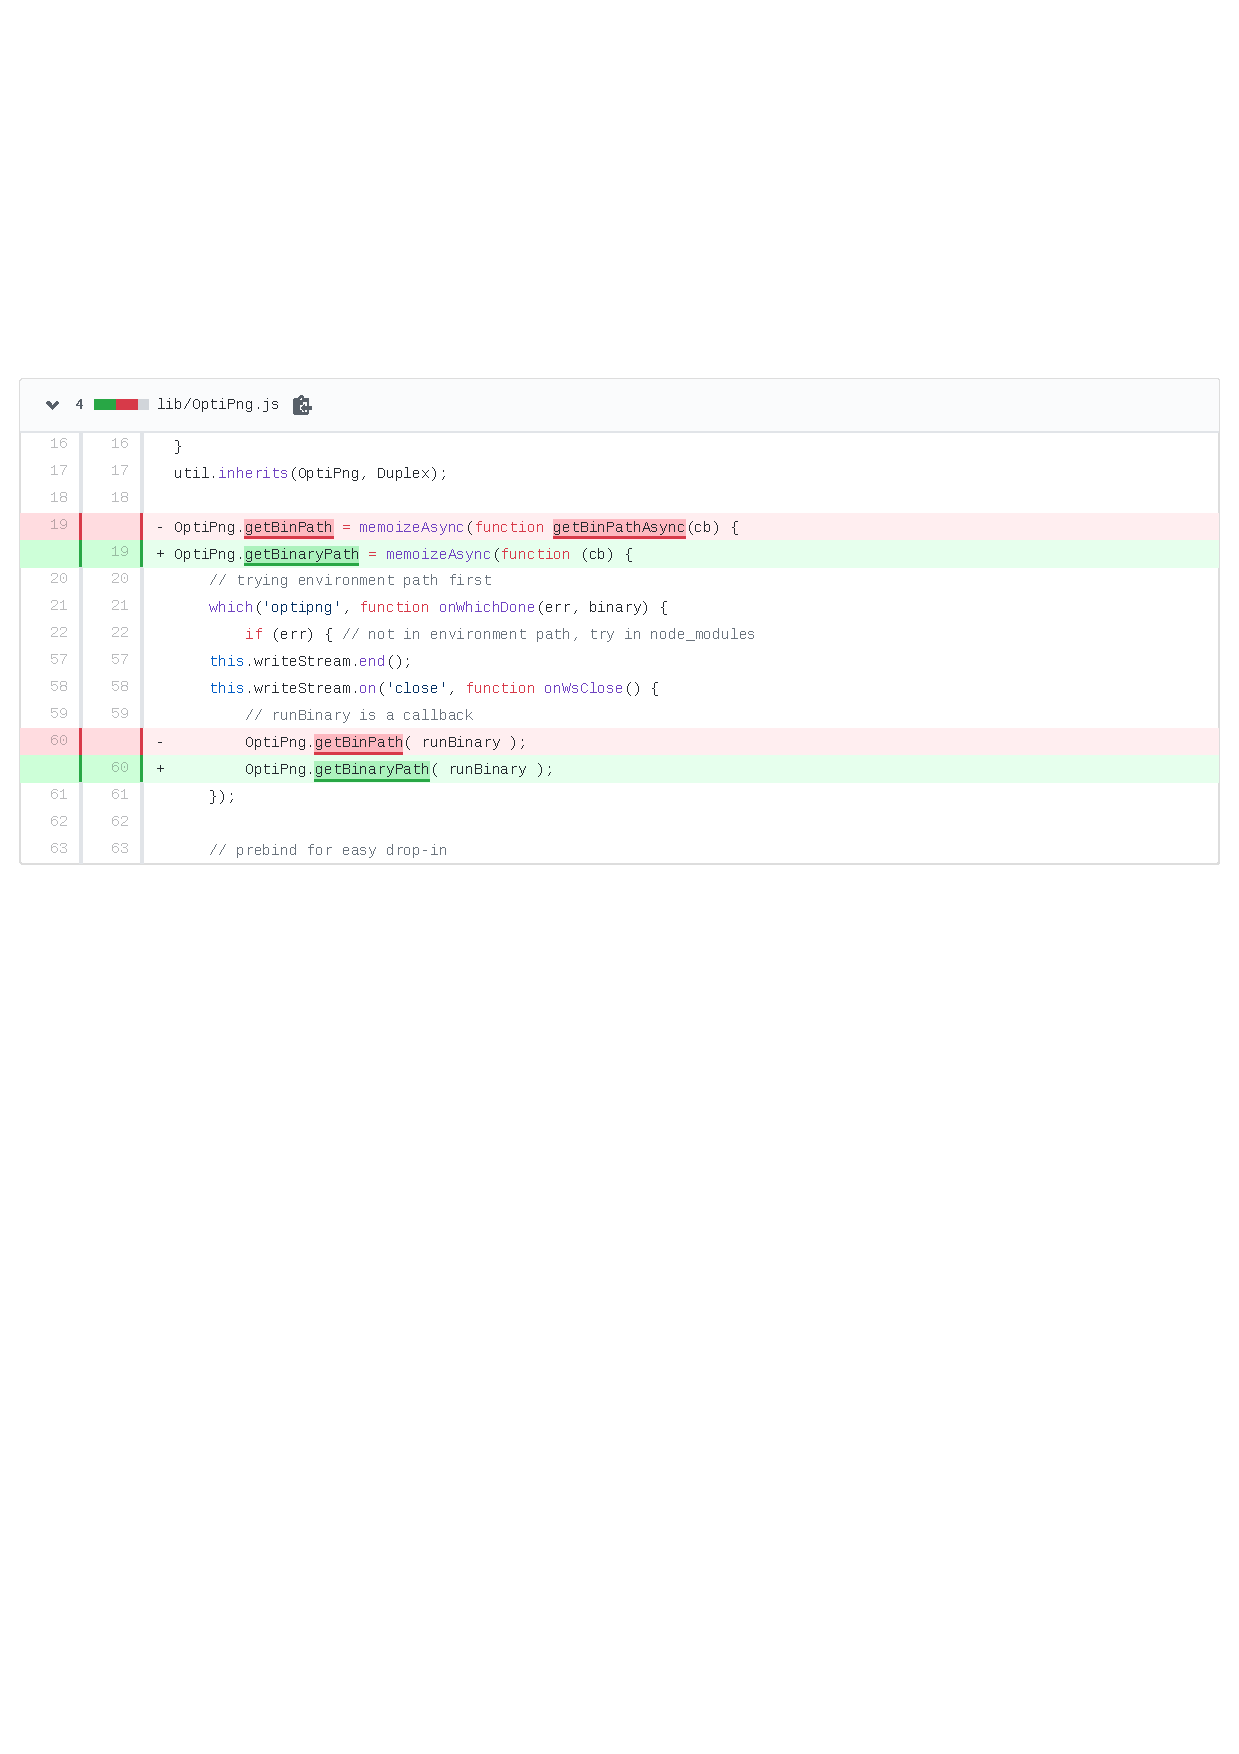
\includegraphics[scale=0.65]{figuras/bc_example.pdf}
    \caption{\textit{Commit} que corrigiu a \textit{breaking change}}
    \label{fig:bc_optipng}
\end{figure}{}

Alterações no código que causam \textit{breaking change} devem ser introduzidas em \textit{releases} versionadas com o incremento do nível \textit{major}, seguindo as especificações do Versionamento Semântico, definidos na Seção \ref{ref-teo:semver}. Assim, um cliente pode especificar se deseja ou não receber as \textit{releases} que contêm \textit{breaking change}. Entretanto, pesquisas relacionadas mostram que as \textit{breaking changes} são introduzidas erroneamente pelos provedores, assim, impactando os clientes. \citeonline{teorical_reference:bc_1} constatou que 9\% das \textit{releases} dos três pacotes com mais dependentes no \textit{npm} introduziram \textit{breaking changes} indevidamente e \citeonline{noregrets2018} apresentou uma ferramenta para detecção de \textit{breaking changes} e também constatou que 9\% das \textit{releases} introduziram \textit{breaking changes} quando não deveriam introduzir.
\daniel{Esses são os que eu coloquei nos trabalhos relacionados}

Além de quantificar as \textit{breaking changes} no ecossistema do \textit{npm}, este trabalho apresenta uma proposta para categorizar essas \textit{breaking changes} e verificar como os clientes se recuperam. Para isso, foi utilizado uma amostra representativa dos clientes no \textit{npm} e, para cada uma de suas \textit{releases}, foi verificado se houve alteração nas \textit{releases} que os clientes aceitavam dos provedores. Então, as versões dos provedores foram resolvidas para a última versão disponível até momento da publicação da \textit{release} do cliente e as \textit{releases} foram executadas através dos \textit{scripts npm install/npm test}. Após, foi feita uma análise manual no código das \textit{releases} que resultaram em erro para confirmar se o erro se tratava de uma \textit{breaking change} ou não. Por fim, foi feita uma análise nos repositórios dos provedores que introduziram as \textit{breaking change} para recuperar informações, tais como, tipo de \textit{breaking change}, tempo que levou até ser consertada, o nível da versão que a \textit{breaking change} foi introduzida/consertada.

Desse modo, o Capítulo \ref{cap:ref-teorico} contém a descrição de todos os termos utilizados ao longo desse trabalho. O Capítulo \ref{cap:qp} contém a motivação e o método para cada uma das questões de pesquisa. O Capítulo \ref{cap:metodologia} descreve sobre a manipulação dos dados que serão utilizados nessa pesquisa\daniel{serão ou foram?}. Por fim, o Capítulo \ref{cap:cronograma} apresenta o cronograma previsto das atividades faltantes para terminar esse trabalho.

% isso estava nos results
%\filipe{o erro sempre se manifesta no cliente, acho que o lance é que você consegue identificar se o erro foi proveniente de uma chamada a uma função do provedor ou do próprio cliente (ou algum outro provedor que não interessa à análise).}

%\filipe{breaking change (defeito no provedor) vs. manifestação da breaking change (manifestação do defeito do provedor no cliente)}